\def\SECTION{3.1 Pairs of Lines and Angles}
\documentclass[aspectratio=169,14pt]{beamer}
\usepackage[T1]{fontenc}
\usepackage{mathpazo}
\usepackage{amsmath,amssymb}
\usepackage{tikz}
\usetikzlibrary{arrows.meta,calc,decorations.pathreplacing}
\definecolor{fblue}{HTML}{1F4E79}
\definecolor{fteal}{HTML}{0F7C7C}
\definecolor{fgold}{HTML}{C9962B}
\definecolor{fred}{HTML}{B3261E}
\definecolor{fink}{HTML}{16233B}
\definecolor{fsoft}{HTML}{EEF3F8}
\definecolor{fgoldsoft}{HTML}{FBF1DC}
\setbeamertemplate{navigation symbols}{}
\setbeamercolor{normal text}{fg=fink}
\setbeamercolor{frametitle}{fg=fblue}
\setbeamerfont{frametitle}{series=\bfseries,size=\Large}
\setbeamercolor{structure}{fg=fteal}
\setbeamertemplate{itemize item}{\color{fteal}$\blacktriangleright$}
\setbeamertemplate{frametitle}{\vspace{6pt}\insertframetitle\par\vspace{-2pt}{\color{fgold}\rule{2.2cm}{2pt}}}
\setbeamertemplate{footline}{\hspace{0.6cm}{\color{fblue}\scriptsize\bfseries Fang\textcolor{fteal}{Math}}\hfill{\scriptsize\color{gray}\SECTION\quad\insertframenumber}\hspace{0.6cm}\vspace{6pt}}
\newcommand{\key}[1]{{\color{fteal}\textbf{#1}}}
\newcommand{\ans}[1]{\colorbox{fgoldsoft}{\color{fink}\ensuremath{#1}}}
\newcommand{\warn}[1]{\begin{beamercolorbox}[sep=8pt,rounded=true]{warnbox}{\color{fred}\textbf{Watch out!}}\enskip #1\end{beamercolorbox}}
\setbeamercolor{warnbox}{bg=fred!8,fg=fink}
\setbeamercolor{turnbox}{bg=fgoldsoft,fg=fink}
\setbeamercolor{defbox}{bg=fsoft,fg=fink}
\newcommand{\defn}[1]{\begin{beamercolorbox}[sep=8pt,rounded=true]{defbox}#1\end{beamercolorbox}}
\newenvironment{yourturn}{\begin{beamercolorbox}[sep=10pt,rounded=true]{turnbox}{\color{fgold}\Large\bfseries Your turn!}\quad{\small Pause the video and try it.}\par\medskip}{\end{beamercolorbox}}
\newcommand{\titleframe}[3]{%
\begin{frame}[plain]
\begin{tikzpicture}[remember picture,overlay]
\fill[fblue] (current page.north west) rectangle ([yshift=-0.9cm]current page.north east);
\node[anchor=west,text=white,font=\bfseries] at ([xshift=0.6cm,yshift=-0.45cm]current page.north west) {Fang\textcolor{fgold}{Math}};
\node[anchor=east,text=white,font=\small] at ([xshift=-0.6cm,yshift=-0.45cm]current page.north east) {Geometry $\cdot$ Chapter \CHNO};
\end{tikzpicture}
\vfill
{\color{fteal}\large\bfseries #1}\par\medskip
{\color{fblue}\fontsize{30}{34}\selectfont\bfseries #2}\par\medskip
{\color{fgold}\rule{3cm}{3pt}}\par\bigskip
{\large #3}
\vfill
{\small\color{gray} fangmath.com $\cdot$ YouTube @fangmathcom}
\end{frame}}
\newcommand{\closeframe}[1]{%
\begin{frame}{Remember}
#1
\vfill
\begin{center}{\color{fblue}\large\bfseries Now practice at your level:}\par\smallskip
{\Large\color{fteal}\bfseries fangmath.com} \enskip{\color{gray}$\to$ Geometry $\to$ Chapter \CHNO}\end{center}
\end{frame}}

\usepackage{pgfplots}\pgfplotsset{compat=1.17}
\newcommand{\grid}[4]{\draw[step=1,gray!25] (#1,#2) grid (#3,#4);\draw[-{Stealth},gray] (#1,0)--(#3+0.3,0) node[right]{\small$x$};\draw[-{Stealth},gray] (0,#2)--(0,#4+0.3) node[above]{\small$y$};}
\def\CHNO{3}
\usetikzlibrary{angles,quotes}
\begin{document}
\titleframe{Lesson 3.1}{Pairs of Lines \& Angles}{Parallel, skew, and the angles a transversal makes}
\begin{frame}{Three ways two lines can relate}
\onslide<1->{\key{Intersecting}: the lines meet in one point.}\par\medskip
\onslide<2->{\key{Parallel}: coplanar and \textbf{never} meet.}\par\medskip
\onslide<3->{\key{Skew}: \textbf{not} coplanar and never meet --- only in 3D.}\par\medskip
\end{frame}
\begin{frame}{Look at a box}
\begin{columns}[c]\begin{column}{0.44\textwidth}\centering 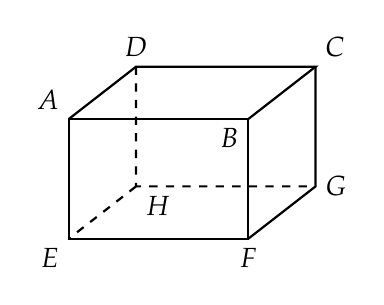
\begin{tikzpicture}[scale=0.95]\draw[thick] (0,0) rectangle (2.4,1.6);\draw[thick] (0,1.6)--(0.9,2.3)--(3.3,2.3)--(2.4,1.6);\draw[thick] (3.3,2.3)--(3.3,0.7)--(2.4,0);\draw[thick,dashed] (0.9,2.3)--(0.9,0.7)--(3.3,0.7) (0.9,0.7)--(0,0);\node[above left] at (0,1.6){$A$};\node[below left] at (2.4,1.6){$B$};\node[above right] at (3.3,2.3){$C$};\node[above] at (0.9,2.3){$D$};\node[below left] at (0,0){$E$};\node[below] at (2.4,0){$F$};\node[right] at (3.3,0.7){$G$};\node[below right] at (0.9,0.7){$H$};\end{tikzpicture}\end{column}\begin{column}{0.54\textwidth}\onslide<1->{$\overleftrightarrow{AB}$ and $\overleftrightarrow{DC}$: \ans{\text{parallel}}}\par\medskip
\onslide<2->{$\overleftrightarrow{AB}$ and $\overleftrightarrow{BF}$: \ans{\text{intersecting}}}\par\medskip
\onslide<3->{$\overleftrightarrow{AB}$ and $\overleftrightarrow{CG}$: \ans{\text{skew}}}\par\medskip
\onslide<4->{plane $ABCD \parallel$ plane $EFGH$}\par\medskip\end{column}\end{columns}
\end{frame}
\begin{frame}{A transversal makes 8 angles}
\begin{columns}[c]\begin{column}{0.44\textwidth}\centering 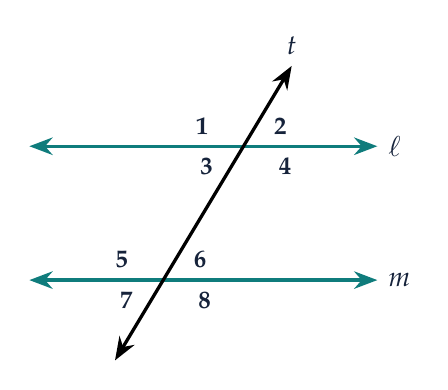
\begin{tikzpicture}[scale=0.85]\draw[very thick,fteal,{Stealth}-{Stealth}] (-2.6,1)--(2.6,1) node[right,fink]{$\ell$};\draw[very thick,fteal,{Stealth}-{Stealth}] (-2.6,-1)--(2.6,-1) node[right,fink]{$m$};\draw[very thick,{Stealth}-{Stealth}] (-1.32,-2.2)--(1.32,2.2) node[above,fink]{$t$};\node[font=\small\bfseries,text=fink] at (-0.02,1.30){1};\node[font=\small\bfseries,text=fink] at (1.15,1.30){2};\node[font=\small\bfseries,text=fink] at (0.05,0.70){3};\node[font=\small\bfseries,text=fink] at (1.22,0.70){4};\node[font=\small\bfseries,text=fink] at (-1.22,-0.70){5};\node[font=\small\bfseries,text=fink] at (-0.05,-0.70){6};\node[font=\small\bfseries,text=fink] at (-1.15,-1.30){7};\node[font=\small\bfseries,text=fink] at (0.02,-1.30){8};\end{tikzpicture}\end{column}\begin{column}{0.54\textwidth}\onslide<1->{A \key{transversal} $t$ crosses two lines and makes \key{8 angles}.}\par\medskip
\onslide<2->{Angles $1$--$4$ at the top crossing, $5$--$8$ at the bottom crossing.}\par\medskip
\onslide<3->{\key{Interior}: between the two lines. \quad \key{Exterior}: outside them.}\par\medskip\end{column}\end{columns}
\end{frame}
\begin{frame}{Name the angle pairs}
\begin{columns}[c]\begin{column}{0.44\textwidth}\centering 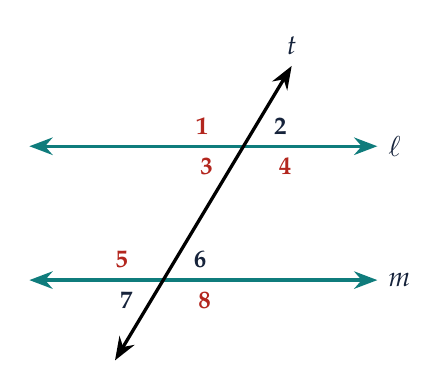
\begin{tikzpicture}[scale=0.85]\draw[very thick,fteal,{Stealth}-{Stealth}] (-2.6,1)--(2.6,1) node[right,fink]{$\ell$};\draw[very thick,fteal,{Stealth}-{Stealth}] (-2.6,-1)--(2.6,-1) node[right,fink]{$m$};\draw[very thick,{Stealth}-{Stealth}] (-1.32,-2.2)--(1.32,2.2) node[above,fink]{$t$};\node[font=\small\bfseries,text=fred] at (-0.02,1.30){1};\node[font=\small\bfseries,text=fink] at (1.15,1.30){2};\node[font=\small\bfseries,text=fred] at (0.05,0.70){3};\node[font=\small\bfseries,text=fred] at (1.22,0.70){4};\node[font=\small\bfseries,text=fred] at (-1.22,-0.70){5};\node[font=\small\bfseries,text=fink] at (-0.05,-0.70){6};\node[font=\small\bfseries,text=fink] at (-1.15,-1.30){7};\node[font=\small\bfseries,text=fred] at (0.02,-1.30){8};\end{tikzpicture}\end{column}\begin{column}{0.54\textwidth}\onslide<1->{\key{Corresponding}: same position, e.g. $\angle 1$ and $\angle 5$}\par\medskip
\onslide<2->{\key{Alternate interior}: inside, opposite sides, e.g. $\angle 4$ and $\angle 5$}\par\medskip
\onslide<3->{\key{Alternate exterior}: outside, opposite sides, e.g. $\angle 1$ and $\angle 8$}\par\medskip
\onslide<4->{\key{Same-side interior}: inside, same side, e.g. $\angle 3$ and $\angle 5$}\par\medskip\end{column}\end{columns}
\end{frame}
\begin{frame}{Watch out}
\onslide<1->{\warn{Two lines that never meet are not always parallel. If no plane contains both, they are \textbf{skew}.}}\par\medskip
\end{frame}
\begin{frame}{}
\begin{columns}[c]\begin{column}{0.6\textwidth}\begin{yourturn}Name each pair: \ (a) $\angle 2$ and $\angle 6$ \quad (b) $\angle 3$ and $\angle 6$ \quad (c) $\angle 4$ and $\angle 6$\end{yourturn}\par\medskip
\onslide<2->{(a) \ans{\text{corresponding}} \\ (b) \ans{\text{alternate interior}} \\ (c) \ans{\text{same-side interior}}}\par\medskip\end{column}\begin{column}{0.38\textwidth}\centering 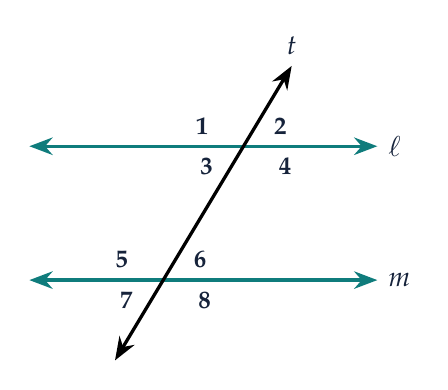
\begin{tikzpicture}[scale=0.85]\draw[very thick,fteal,{Stealth}-{Stealth}] (-2.6,1)--(2.6,1) node[right,fink]{$\ell$};\draw[very thick,fteal,{Stealth}-{Stealth}] (-2.6,-1)--(2.6,-1) node[right,fink]{$m$};\draw[very thick,{Stealth}-{Stealth}] (-1.32,-2.2)--(1.32,2.2) node[above,fink]{$t$};\node[font=\small\bfseries,text=fink] at (-0.02,1.30){1};\node[font=\small\bfseries,text=fink] at (1.15,1.30){2};\node[font=\small\bfseries,text=fink] at (0.05,0.70){3};\node[font=\small\bfseries,text=fink] at (1.22,0.70){4};\node[font=\small\bfseries,text=fink] at (-1.22,-0.70){5};\node[font=\small\bfseries,text=fink] at (-0.05,-0.70){6};\node[font=\small\bfseries,text=fink] at (-1.15,-1.30){7};\node[font=\small\bfseries,text=fink] at (0.02,-1.30){8};\end{tikzpicture}\end{column}\end{columns}
\end{frame}
\closeframe{\begin{itemize}\setlength\itemsep{8pt}
\item Lines can be \key{intersecting}, \key{parallel} or \key{skew}.
\item A \key{transversal} makes 8 angles.
\item Pairs: \key{corresponding}, \key{alternate interior}, \key{alternate exterior}, \key{same-side interior}.
\end{itemize}}
\end{document}
